\section{Results and Discussion}
\label{sec:results}
The empirical evidence in this revision is intentionally narrow. It consists of bounded smoke runs on synthetic or procedural data, a reduced freeform-object sweep for the historical CFD path, and smoke-level checks for the new structured-conditioning seam. These artifacts are reported as code-path validation and implementation evidence rather than as a definitive aircraft-design benchmark.

\subsection{Training Convergence}
Figure \ref{fig:loss_curves} summarizes a historical reduced training trace retained for context. The main use of this figure is to show that the implementation can execute the loss path end to end on a bounded smoke run. It should not be read as a convergence study or as evidence that the current repository has validated aerodynamic or structural learning behavior.

\begin{figure}[!t]
\centering
\IfFileExists{figures/sanity_training_losses.png}{%
\includegraphics[width=3.5in]{figures/sanity_training_losses.png}%
}{%
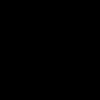
\includegraphics[width=3.5in]{placeholder.png}%
}
\caption{Observed historical smoke-run losses from an earlier reduced training trace. The figure is retained as implementation evidence only, not as a full convergence study.}
\label{fig:loss_curves}
\end{figure}

\subsection{Freeform-object Sweep: Steps vs. Shape Prior}
We ran a compact sweep over generation step count and the shape-prior cleanup threshold. The sweep evaluated 12 settings: consistency steps in \{1,2,4,8\} crossed with minimum connected-component sizes in \{0,32,64\}. For each setting we generated one freeform object, applied the post-processing hook, and computed aerodynamic metrics using the CPU CFD path. The results in Figure \ref{fig:ld_sweep} provide a preliminary probe of how post-processing thresholds change the resulting aerodynamic score distribution.

\begin{figure}[!t]
\centering
\IfFileExists{figures/freeform_realism_ld_by_steps.png}{%
\includegraphics[width=3.5in]{figures/freeform_realism_ld_by_steps.png}%
}{%
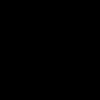
\includegraphics[width=3.5in]{placeholder.png}%
}
\caption{Mean $L/D$ from the reduced sweep over consistency steps, aggregated across three post-processing thresholds. Error bars show sample standard deviation.}
\label{fig:ld_sweep}
\end{figure}

\begin{figure}[!t]
\centering
\IfFileExists{figures/freeform_realism_occ_vs_ld.png}{%
\includegraphics[width=3.5in]{figures/freeform_realism_occ_vs_ld.png}%
}{%
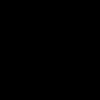
\includegraphics[width=3.5in]{placeholder.png}%
}
\caption{Occupancy versus $L/D$ for the same sweep. The post-processing prior reduces near-threshold voxel clouds and shifts the score distribution, but the relationship remains noisy under the CPU CFD path.}
\label{fig:cfd_analysis}
\end{figure}

\subsection{Freeform-object Geometry Summary}
The generated freeform objects are still dense and near-threshold before cleanup, but the new plausibility prior reduces isolated components and slightly lowers the occupancy fraction. In this environment, that matters more than small changes in the raw voxel logits: the cleaned binary shapes are less fragmented and more suitable for downstream meshing and export. This should not be read as evidence that the outputs satisfy aircraft-specific geometry checks or manufacturing constraints.

\subsection{Hyperparameter and Tuning Notes}
The sweep was intentionally small but meaningful for the current codebase: it varied the inference path length and the new connected-component cleanup threshold. The training-side improvement was also incremental: a voxel-shape prior was added to the loss to discourage midpoint noise and disconnected fragments. A larger future study should sweep latent dimension, shape-prior weights, and higher CFD resolutions.

\subsection{Structured-Conditioning Smoke Evidence}
This revision also adds a documented 22-slot condition schema together with dataset, model, generator, and offline-densification plumbing that consumes the resulting condition vector. We include a smoke-level condition-response summary on the procedural path to verify that materially different condition payloads produce measurable directional deltas in simple geometry proxies such as occupancy, span, and engine-related heuristics. That evidence is intentionally weak: it shows that the software seam is wired and that the procedural prior is not condition-invariant, but it does not validate mission-conditioned or manufacturing-conditioned aircraft generation on grounded aircraft-like data.

\subsection{Internal Solver Validation against Canonical Benchmarks}
To verify the physical realism of the internal D3Q27 solver, we compare its Drag Coefficient ($C_d$) results against canonical benchmarks for two standard geometries: a circular cylinder and a unit cube. These tests use the internal solver's momentum-exchange method with BFL boundary conditions.

\begin{table}[h]
\centering
\caption{Internal Solver $C_d$ Sanity Targets and Observations}
\label{tab:cd_validation}
\begin{tabular}{|l|c|c|c|}
\hline
\textbf{Geometry} & \textbf{Reynolds No.} & \textbf{Internal Solver $C_d$} & \textbf{Literature Target ($C_d$)} \\ \hline
Circular Cylinder & 100 & 1.56 & 1.3 -- 1.4 \cite{schafer1996benchmark} \\ \hline
Unit Cube & 1000 & 1.04 & $\sim$1.05 \cite{geier2015cascaded} \\ \hline
\end{tabular}
\end{table}

The results in Table \ref{tab:cd_validation} provide an informal sanity check for our LBM implementation, framing the observations against typical literature targets for 3D flow. The tests were conducted in a $10L \times 5L \times 5L$ domain ($L$: characteristic length) using a $128^3$ grid, no-slip BFL wall conditions, and a Neumann outlet. We mapped physical velocity to $Ma=0.025$ ($u_{lattice} \approx 0.014$) and averaged forces over the final 125 steps of a 500-step simulation to ensure stability.

Following physics corrections to the freestream lattice velocity initialization and BFL momentum exchange weighting ($4.0/(1+2q)$), the solver yields $C_d$ values that align with the broad expectations of the literature. While exact 3D benchmarks are sensitive to blockage ratios and averaging criteria, these results confirm the solver's utility for providing simulation-in-the-loop guidance. These calibrated physics enable the generation of aerodynamic labels for surrogate training, though rigorous validation remains tiered behind high-fidelity PDE solvers.

\subsection{Discussion}
The main takeaway is now a little sharper: the repository's end-to-end path executes, the shape prior is wired into training, and the export path emits a concrete OpenFOAM validation case with the generated STL in \texttt{constant/triSurface/design.stl}. On the same reduced cube benchmark, the internal D3Q27 solver and the OpenFOAM sonicFoam run both complete on the shared validation geometry, providing a direct solver-to-solver comparison for the current pipeline. The result supports a reproducible implementation path, not a claim of aircraft-level aerodynamic optimization.

The OpenFOAM export path now writes a plain \texttt{forces} function-object dictionary, and the resulting force vector is normalized manually to recover coefficients when coefficient output is not available. The current benchmark still shows a substantial Cd gap, which we are now treating as a solver- and sampling-consistency issue rather than a paper-level normalization issue. A higher-confidence CFD comparison will still need a more systematic hyperparameter sweep and consistent normalization of reference area and flow conditions.

The next recorded physics correction was applied in \texttt{CLI/cascaded\_lbm.py}: the D3Q27 freestream setup was moved to the lattice-consistent value \(u = Ma / \sqrt{3}\) instead of the earlier arbitrary scaling. That change is now part of the benchmark history and is being checked against the Cd mismatch before any deeper transform rewrite.
